% ---------------------------------------------------------------------------- %
\chapter{Configuration of Laboratory Equipment}
\label{chap:labconfig}
% ---------------------------------------------------------------------------- %

This chapter contains supplementary information for configuring the laboratory
equipment used during the project.

% ---------------------------------------------------------------------------- %
\section{HP Arbitrary Waveform Generator}
\label{sec:HPwave}
% ---------------------------------------------------------------------------- %

Configuring the waveform generator consists of two primary parts:

\begin{itemize}\tightlist
    \item
        Making an initial configuration and storing it for later reuse.
    \item
        Restoring that configuration after a power-down event.
\end{itemize}

% ---------------------------------------------------------------------------- %
\subsection{Initial Configuration}
\label{subsec:HPwave:initialConfig}
% ---------------------------------------------------------------------------- %

When   powered  on,   the   user  will   be  greeted   by   the  screen   from
\fref{fig:HPwave:poweron}. The  first  thing  to  do  is  to  set  the  output
impedance  to  \emph{HIGH}  instead  of  \SI{50}{\ohm}. For  this,  enter  the
menu  by  pressing  \emph{Shift}  and \emph{Enter}. Then  scroll  through  the
menu  using the  \emph{>}  button until  encountering  menu item  \emph{D: SYS
MENU},  seen in  \fref{fig:HPwave:sysMenu}. Enter  the  system config  submenu
by  pressing  the  \emph{v}  key. Press   the  same  key  again  for  entering
the  \emph{OUT TERM}  submenu,  as  seen in  \fref{fig:HPwave:outTerm}. Switch
from   \emph{\SI{50}{\ohm}}   (\fref{fig:HPwave:50Ohm})   to   \emph{HIGH   Z}
(\fref{fig:HPwave:highZ}), confirm with the \emph{Enter} key.

Next,  ensure  that   a  square  wave  is  output  (default   is  sine  wave),
configure  the   frequency  to  the  desired   value  (\fref{fig:HPwave:freq},
\SI{256}{\kilo\hertz}   used   in  this   example),   set   the  VPP   voltage
to   \SI{3}{\volt}  (\fref{fig:HPwave:vpp}),   and   offset   the  signal   by
\SI{1.5}{\volt}  (the  system  expects  an  input  between  \SI{0}{\volt}  and
\SI{3}{\volt},  not   \SI{-1.5}{\volt}  and  \SI{+1.5}{\volt}),  as   seen  in
\fref{fig:HPwave:offset}.

Lastly, store  the configuration in  one of the  available slots, as  shown in
\fref{fig:HPwave:store}. This ensures  that this entire process  does not have
to be repeated after each shutdown of the device.

\todo[inline,color=purple!20!white]{%
    Would it  make sense to  arrange the images in  this section more  in line
    with  the text,  given that  this is  more of  a userguide  rather than  a
    scientific document?
}

\begin{figure}
    \centering
    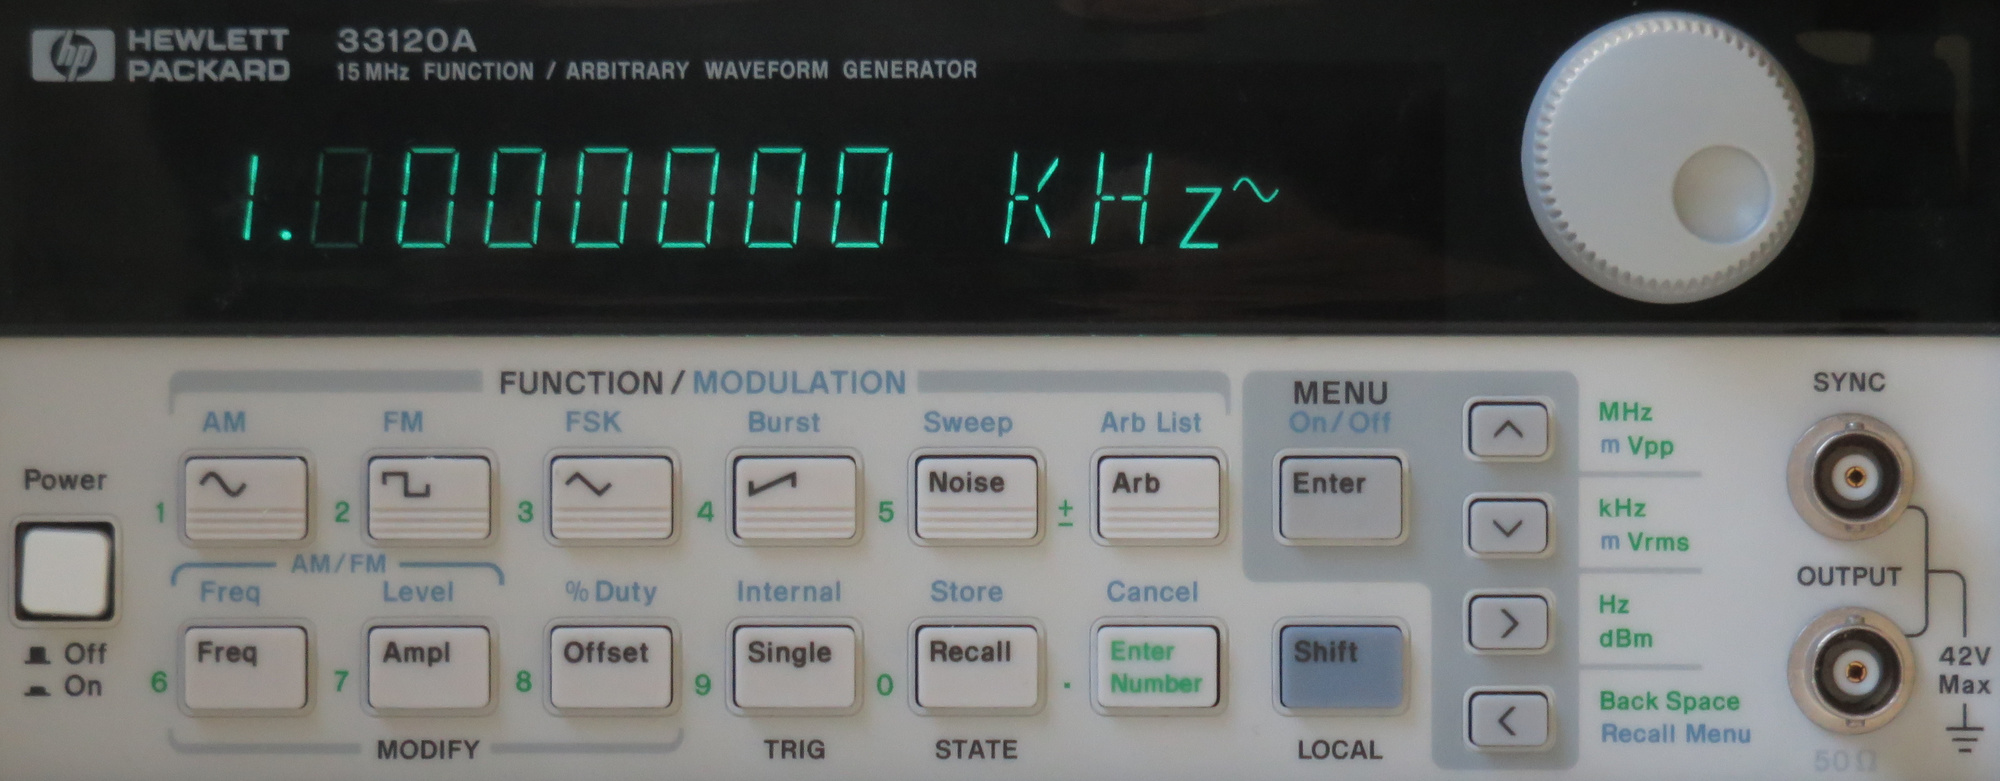
\includegraphics[width=0.67\textwidth]{images/funcGen/funcGen-01.jpg}
    \caption{Initial screen after power-on}
    \label{fig:HPwave:poweron}
\end{figure}

\begin{figure}
    \centering
    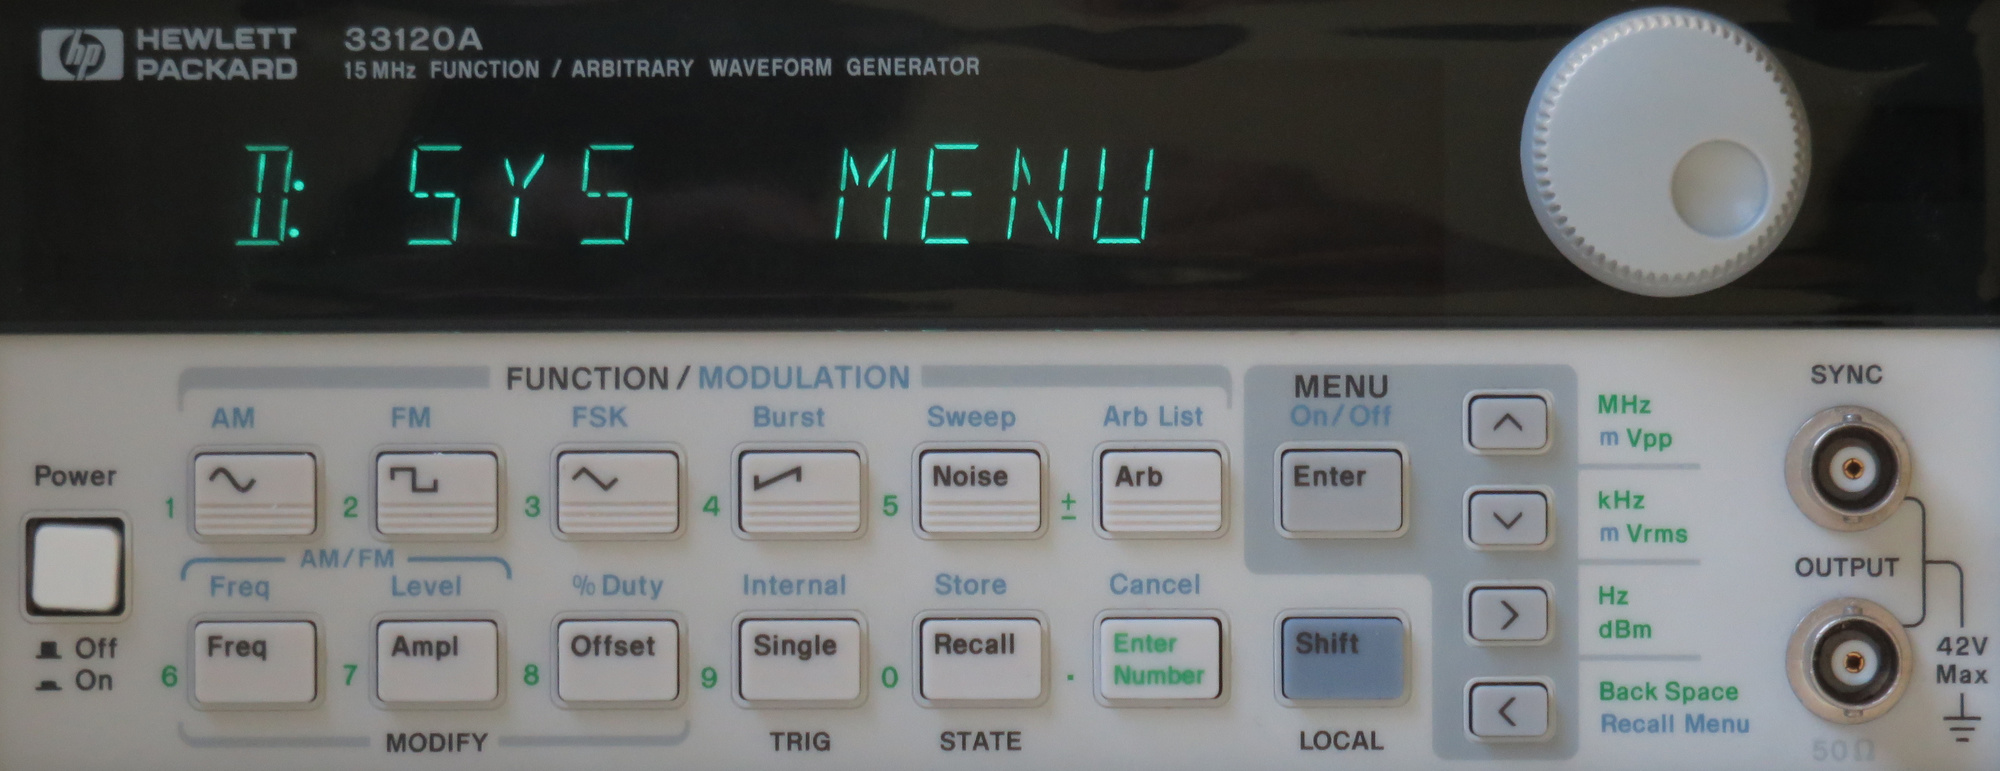
\includegraphics[width=0.67\textwidth]{images/funcGen/funcGen-02.jpg}
    \caption{System config menu}
    \label{fig:HPwave:sysMenu}
\end{figure}

\begin{figure}
    \centering
    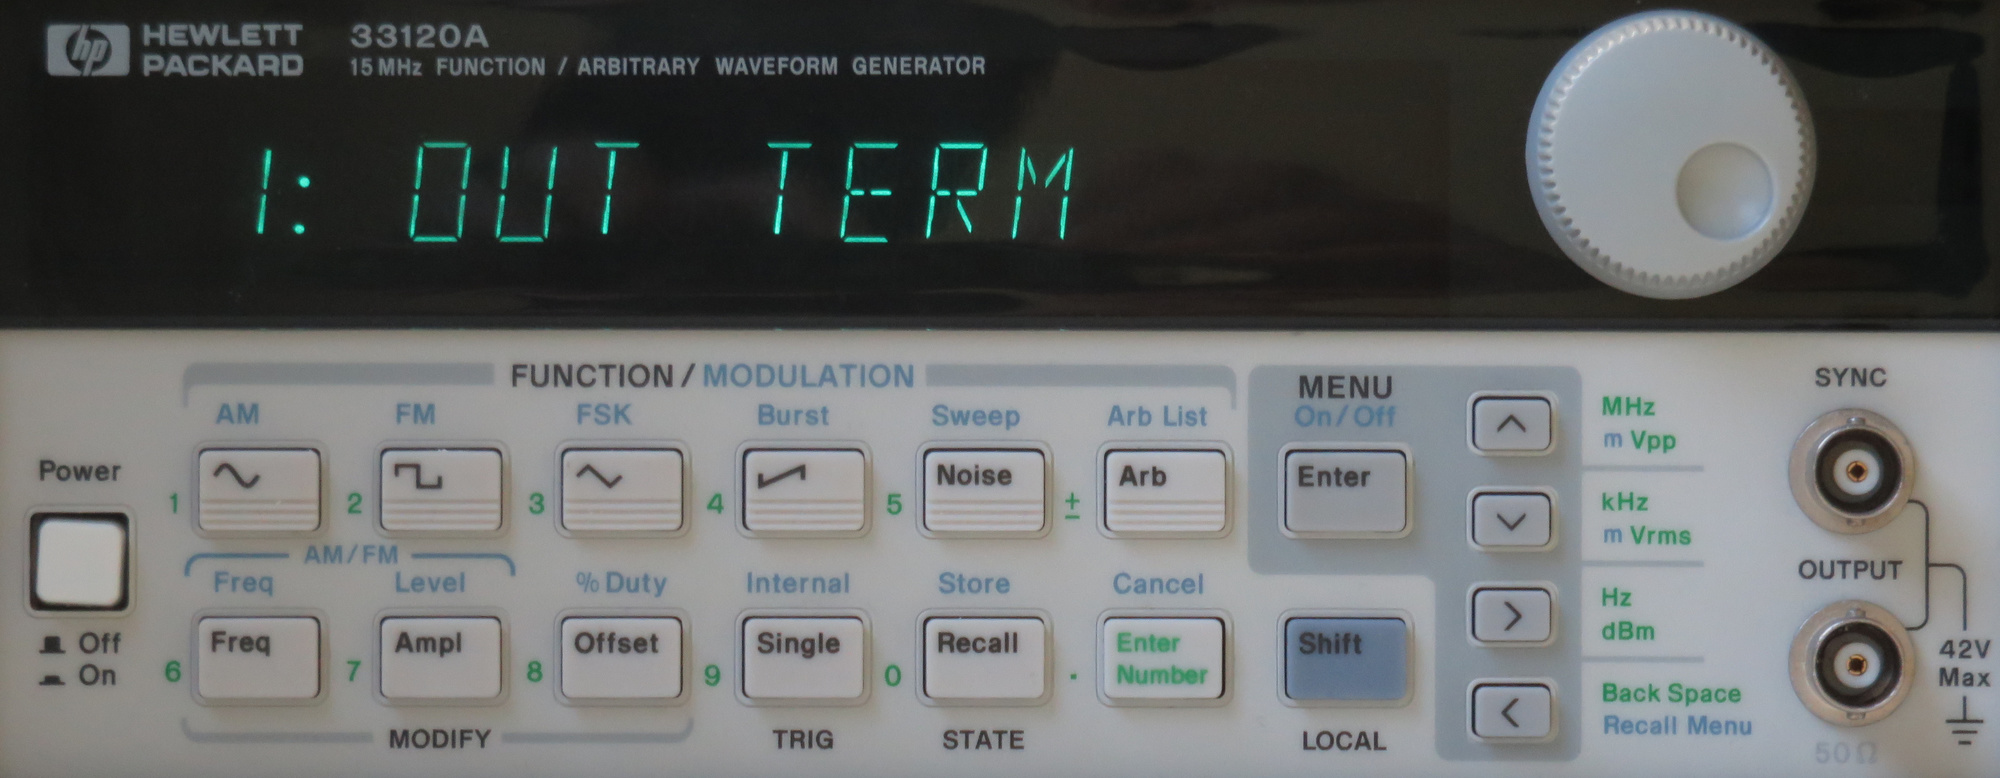
\includegraphics[width=0.67\textwidth]{images/funcGen/funcGen-03.jpg}
    \caption{Select the \emph{OUT TERM} menu item.}
    \label{fig:HPwave:outTerm}
\end{figure}

\begin{figure}
    \centering
    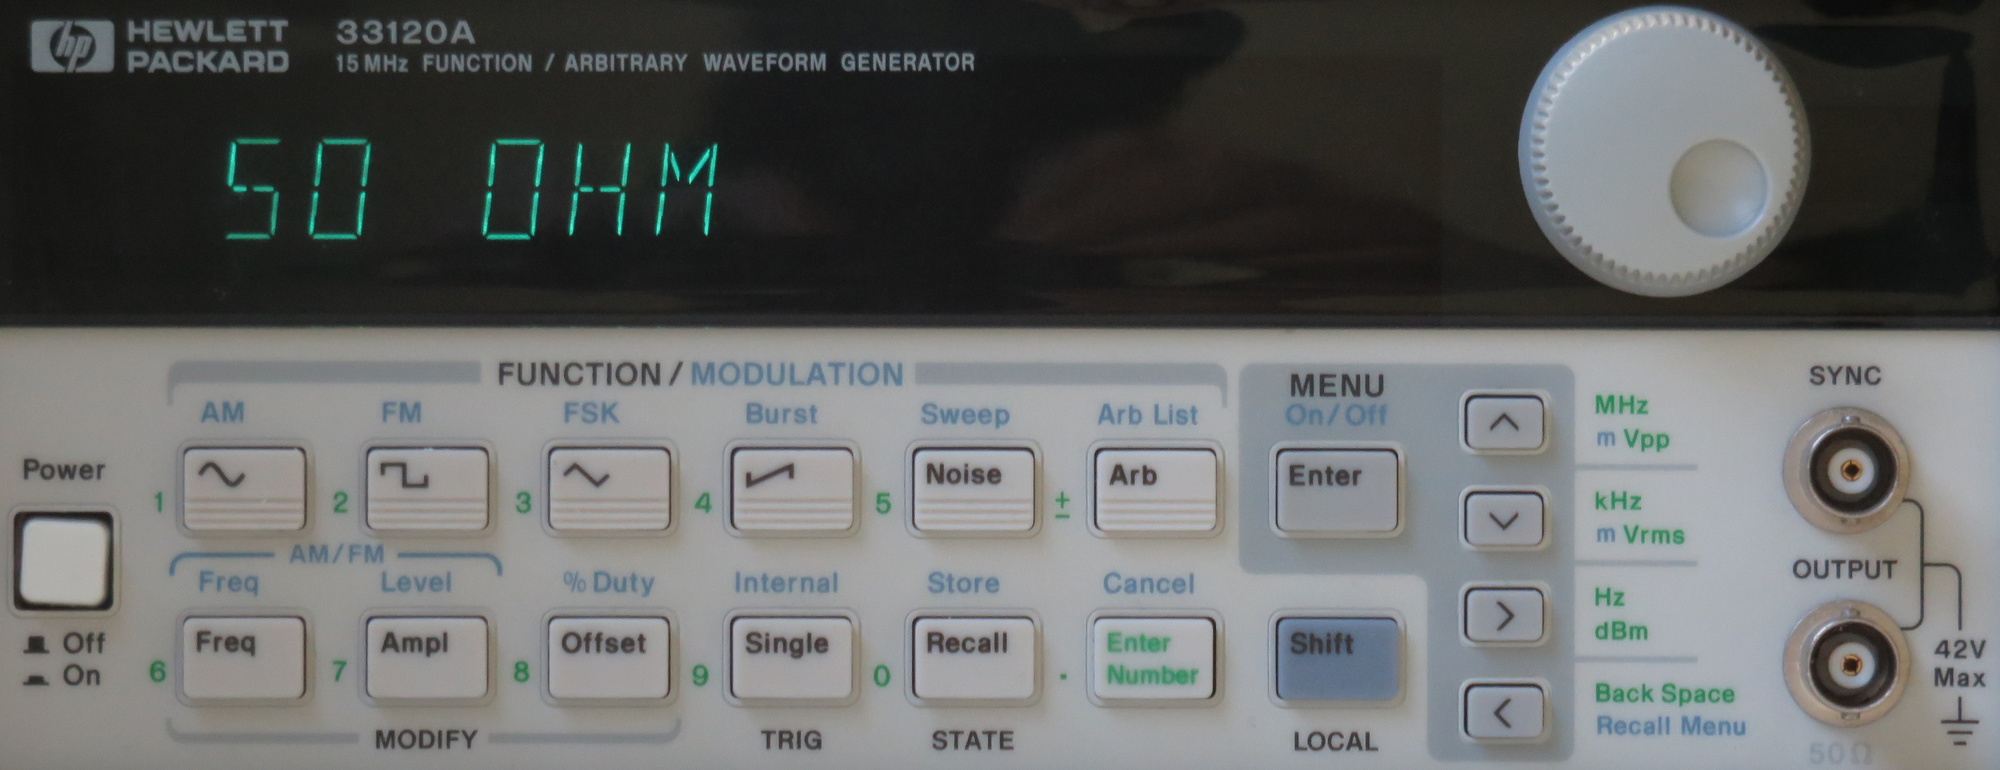
\includegraphics[width=0.67\textwidth]{images/funcGen/funcGen-04.jpg}
    \caption{By default, the output impedance is set to \SI{50}{\ohm}}
    \label{fig:HPwave:50Ohm}
\end{figure}

\begin{figure}
    \centering
    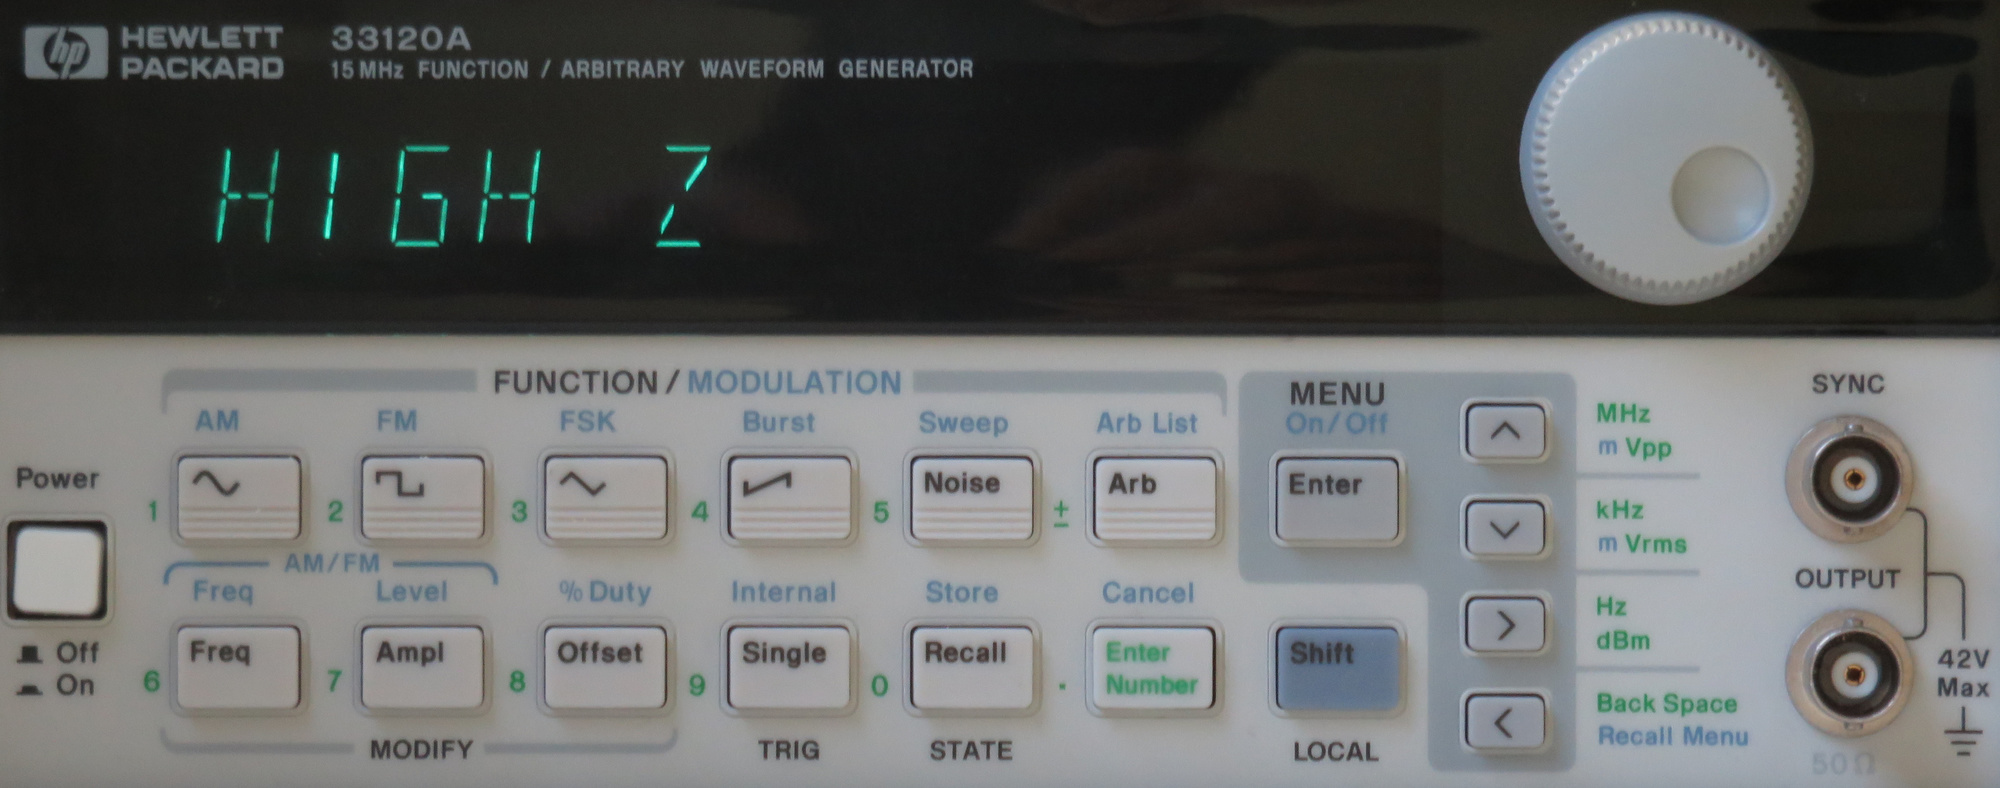
\includegraphics[width=0.67\textwidth]{images/funcGen/funcGen-05.jpg}
    \caption{Setting the output impedance to high}
    \label{fig:HPwave:highZ}
\end{figure}

\begin{figure}
    \centering
    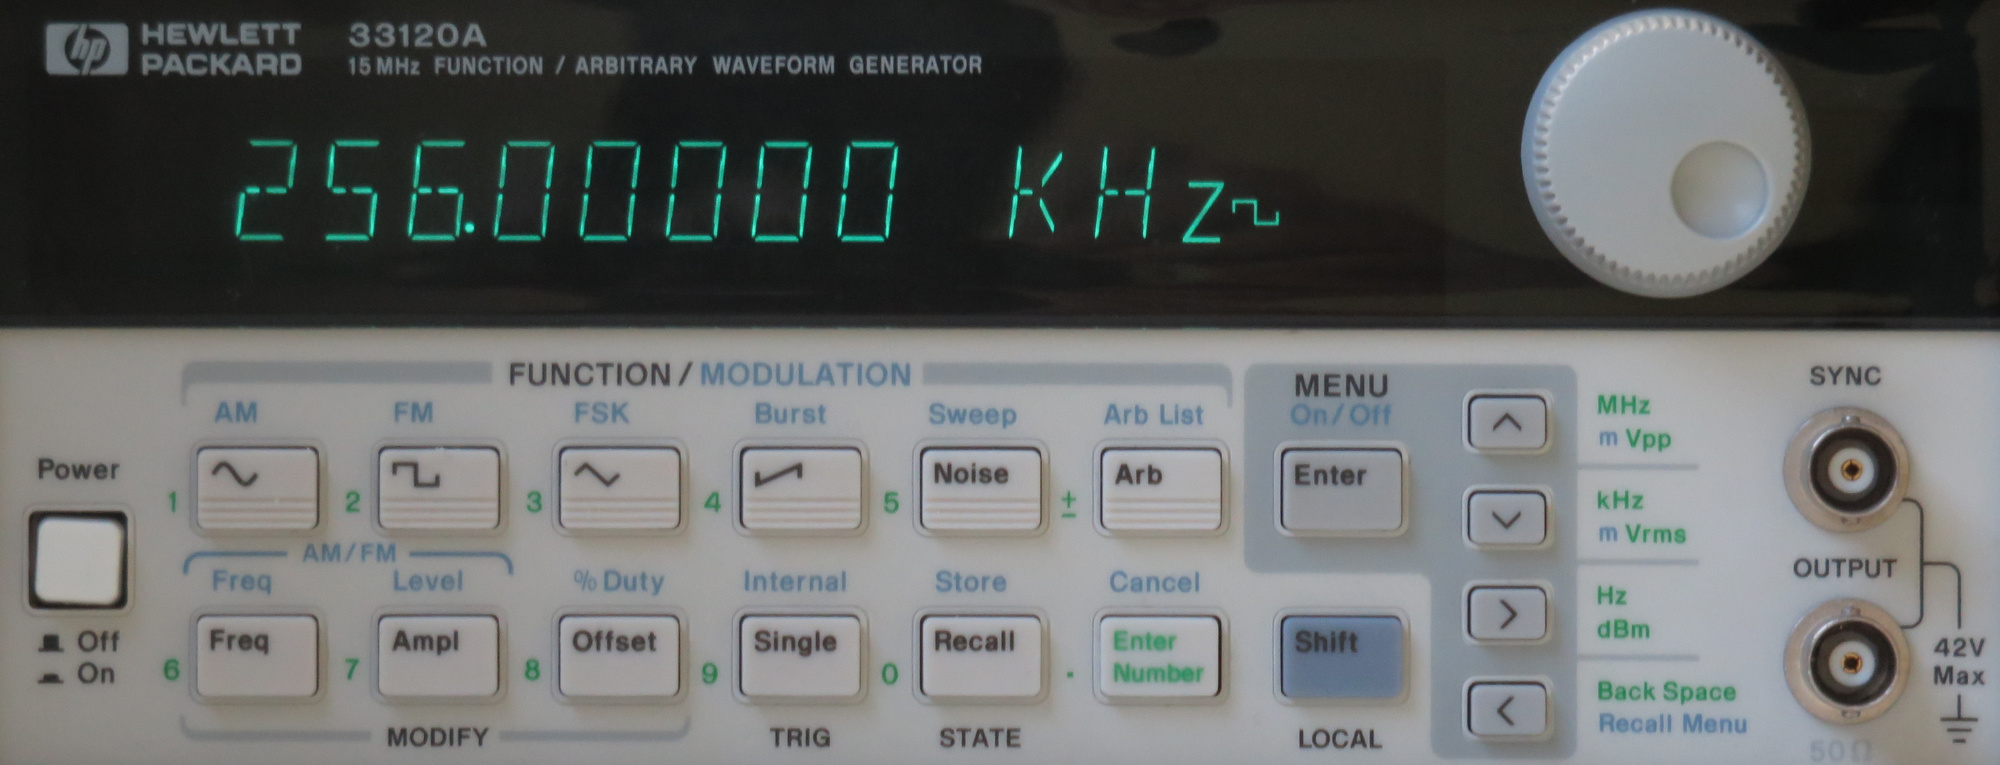
\includegraphics[width=0.67\textwidth]{images/funcGen/funcGen-06.jpg}
    \caption{Frequency configuration screen}
    \label{fig:HPwave:freq}
\end{figure}

\begin{figure}
    \centering
    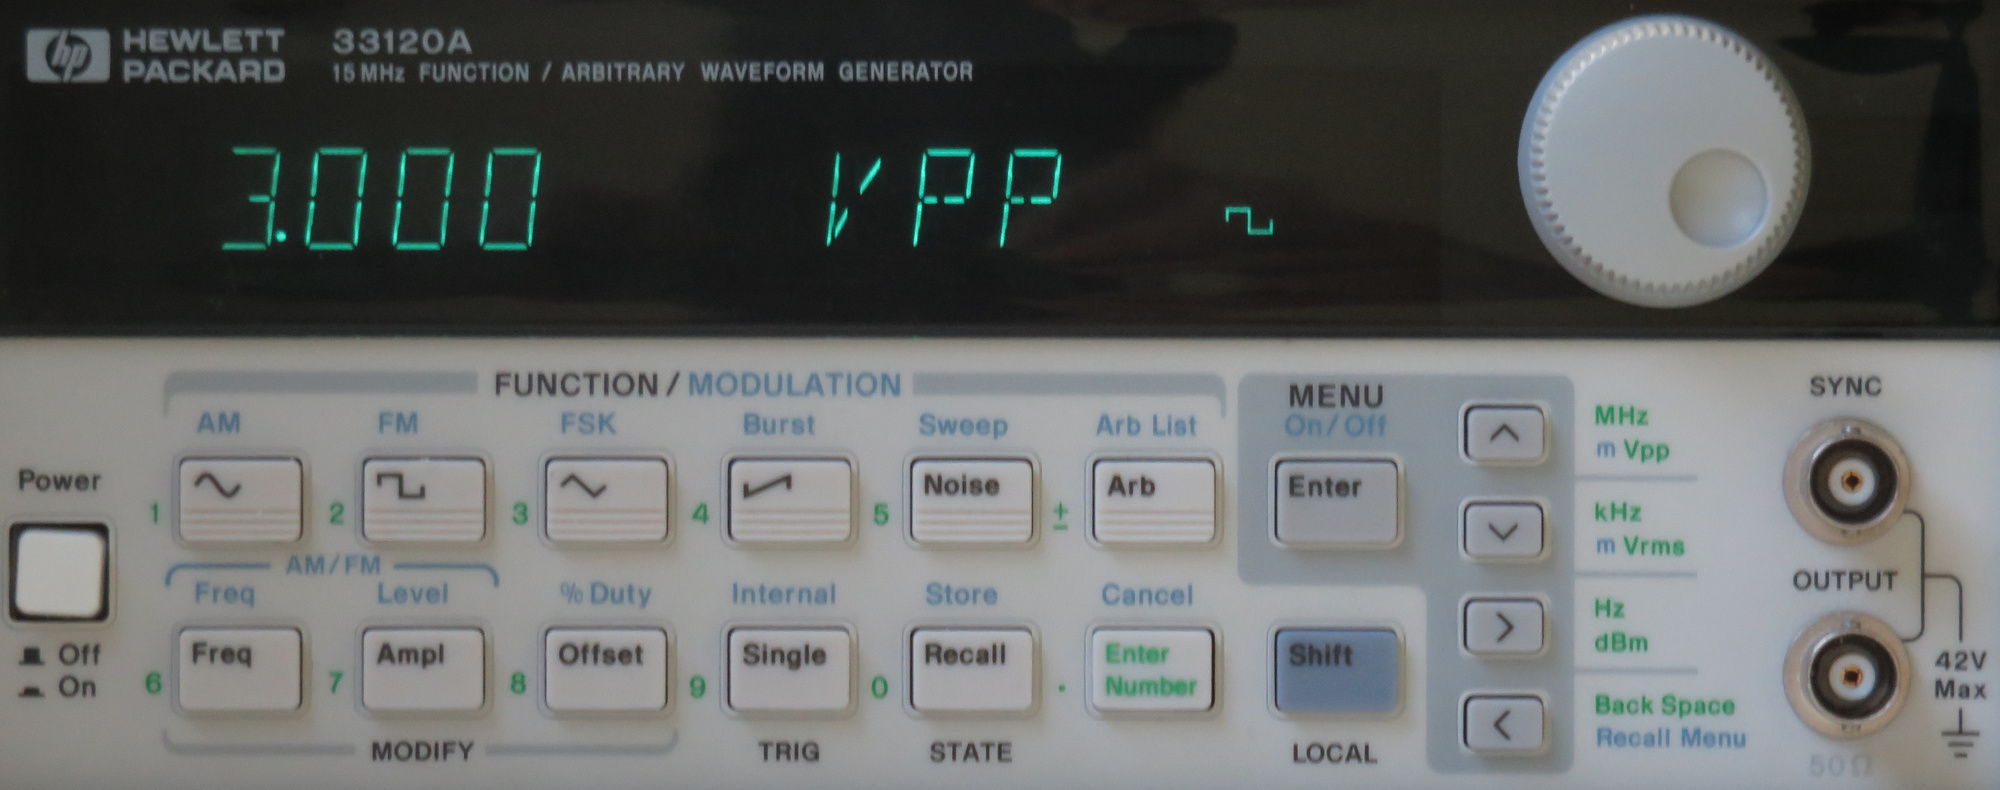
\includegraphics[width=0.67\textwidth]{images/funcGen/funcGen-07.jpg}
    \caption{VPP configuration}
    \label{fig:HPwave:vpp}
\end{figure}

\begin{figure}
    \centering
    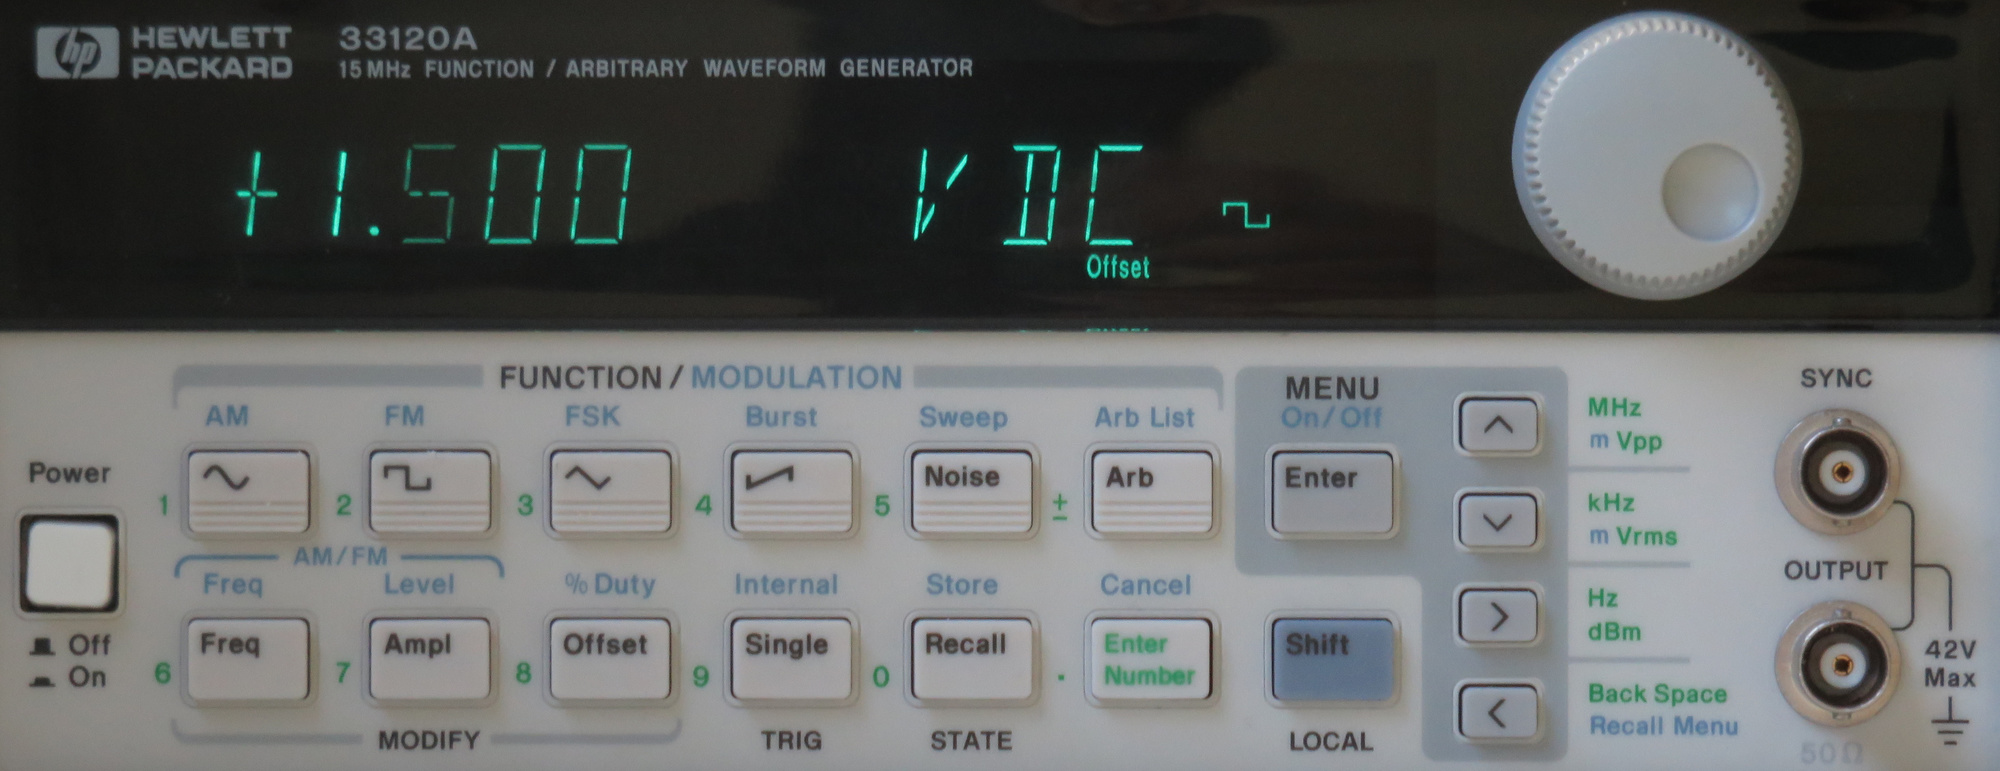
\includegraphics[width=0.67\textwidth]{images/funcGen/funcGen-08.jpg}
    \caption{Offset voltage configuration}
    \label{fig:HPwave:offset}
\end{figure}

\begin{figure}
    \centering
    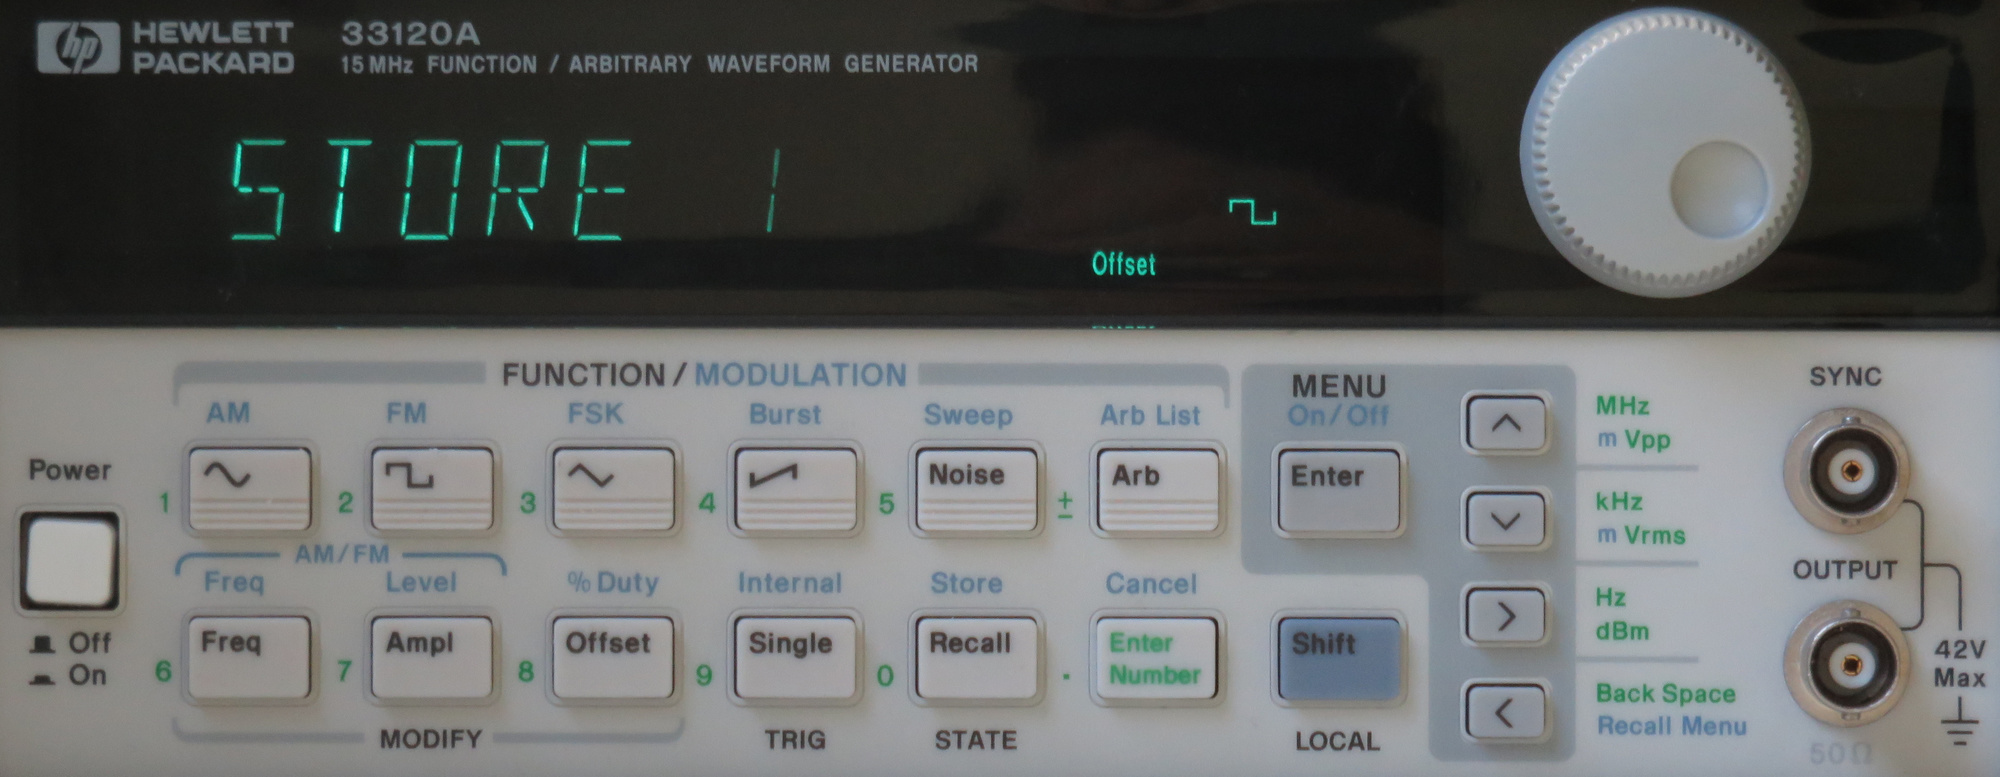
\includegraphics[width=0.67\textwidth]{images/funcGen/funcGen-09.jpg}
    \caption{Storing the configuration in slot 1}
    \label{fig:HPwave:store}
\end{figure}


% ---------------------------------------------------------------------------- %
\clearpage
\subsection{Restoring Configuration}
\label{subsec:HPwave:restoringConfig}
% ---------------------------------------------------------------------------- %

For restoring from a saved configuration, press \emph{RECALL}, select the slot
to be  restored (slot 1  in \fref{fig:HPwave:recall}) and confirm  by pressing
\emph{ENTER}.  The device should now be set to the saved configuration again.

%\begin{figure}
%    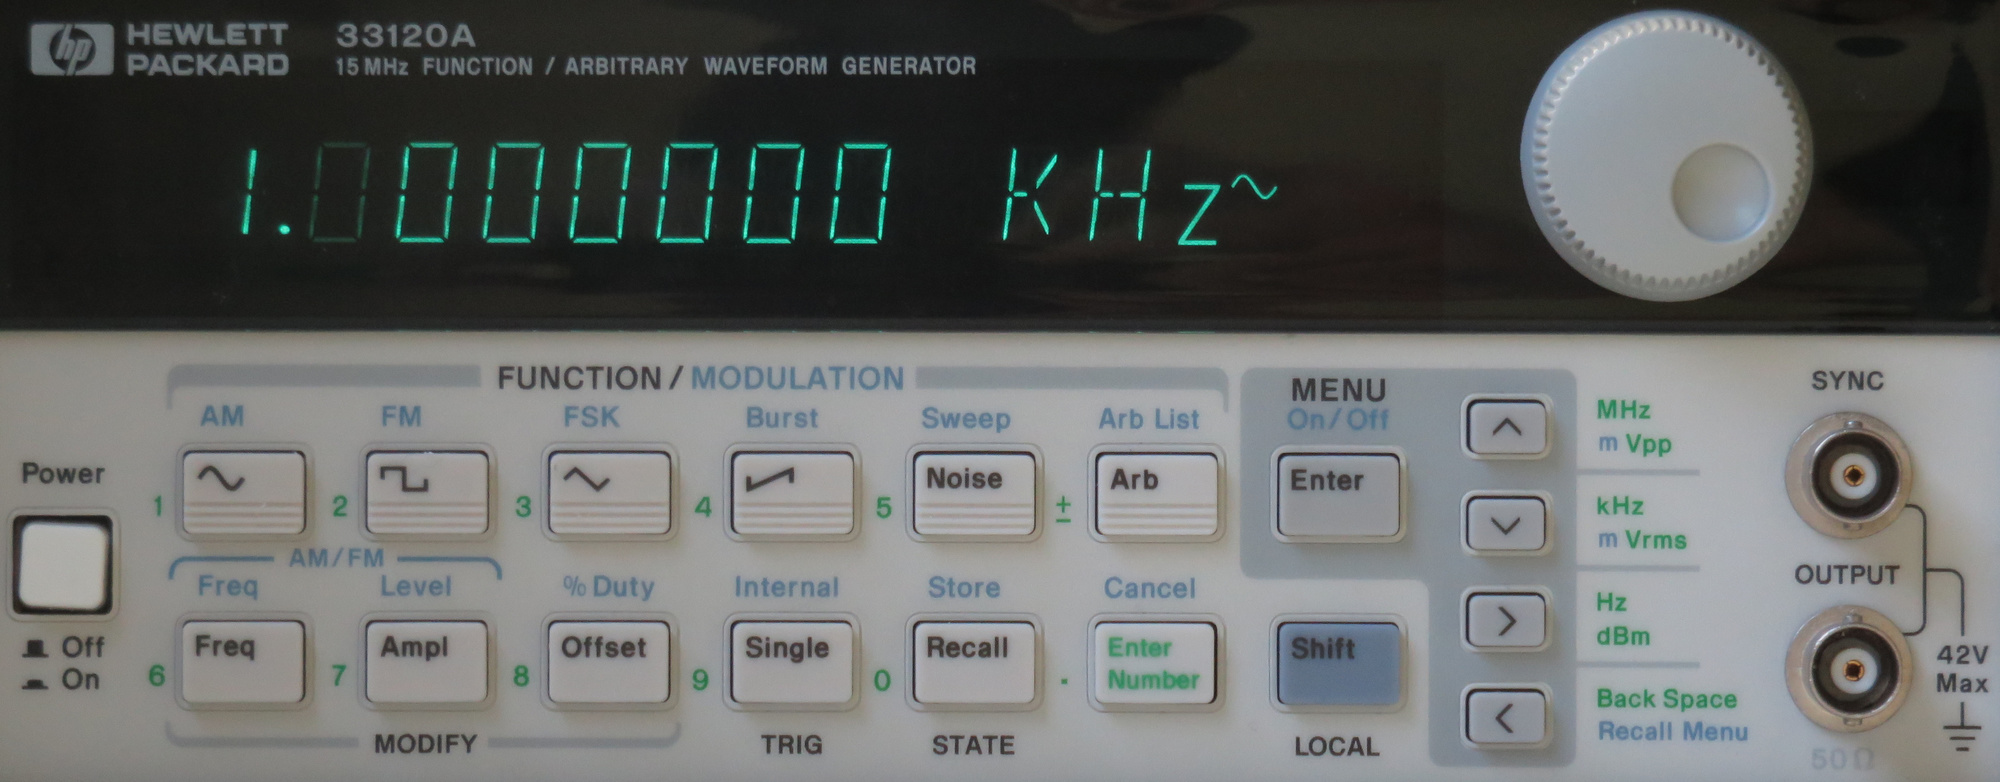
\includegraphics[width=0.67\textwidth]{images/funcGen/funcGen-10.jpg}
%    \caption{Initial screen after power-on}
%    \label{fig:HPwave:poweron}
%\end{figure}

\begin{figure}
    \centering
    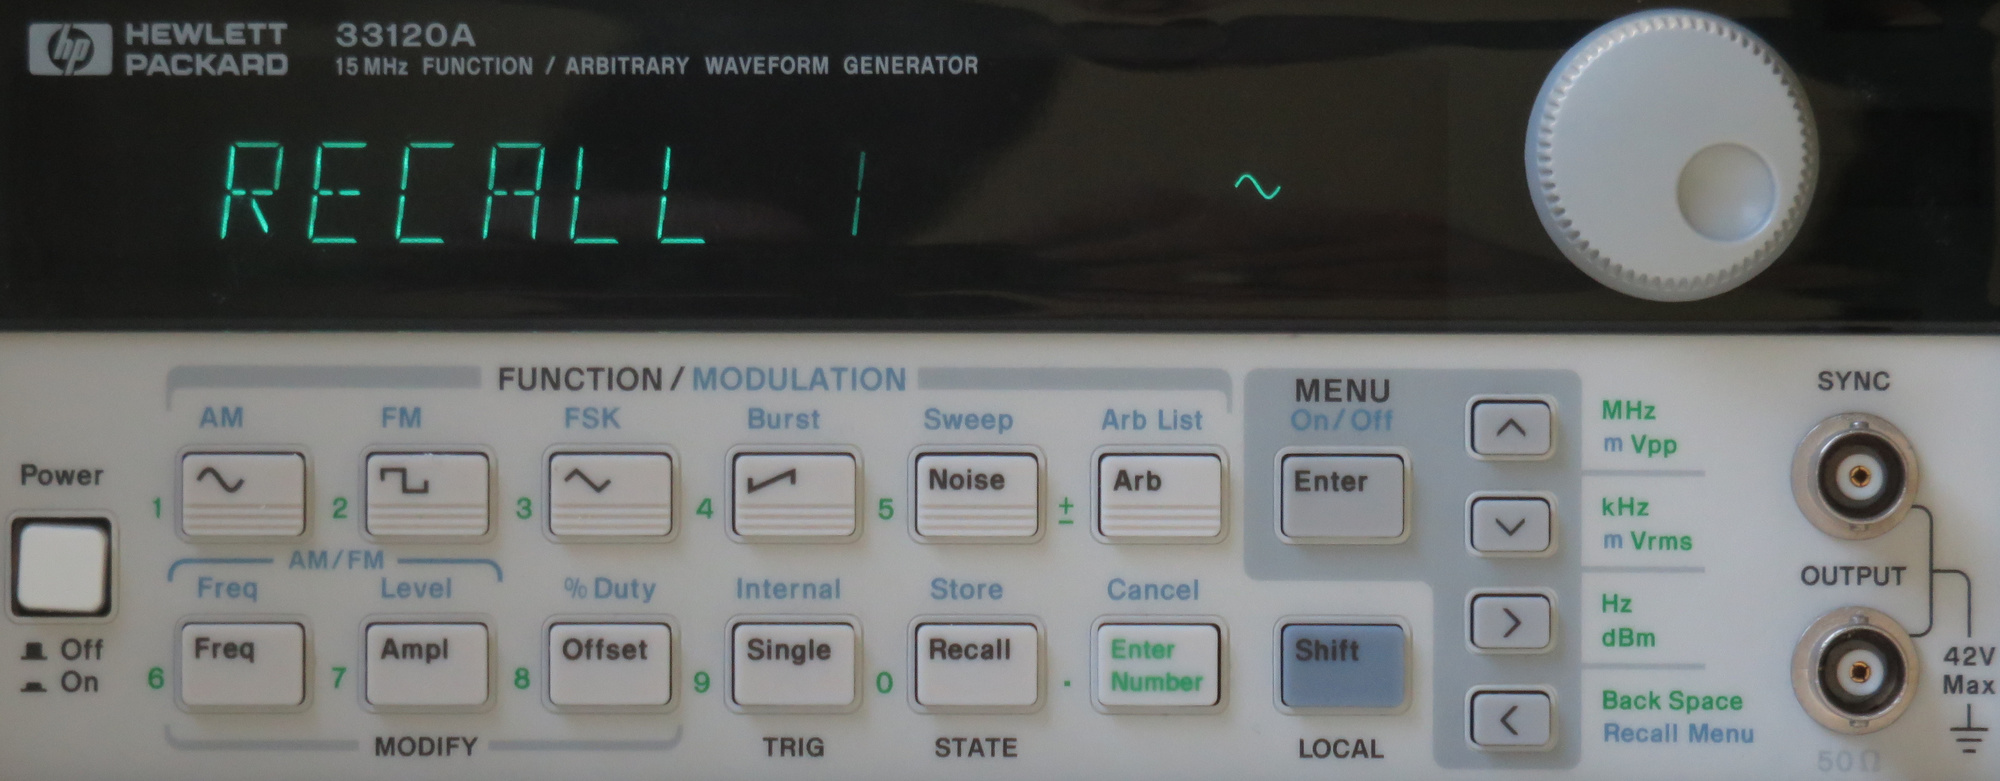
\includegraphics[width=0.67\textwidth]{images/funcGen/funcGen-11.jpg}
    \caption{Initial screen after power-on}
    \label{fig:HPwave:recall}
\end{figure}

%\begin{figure}
    \centering
%    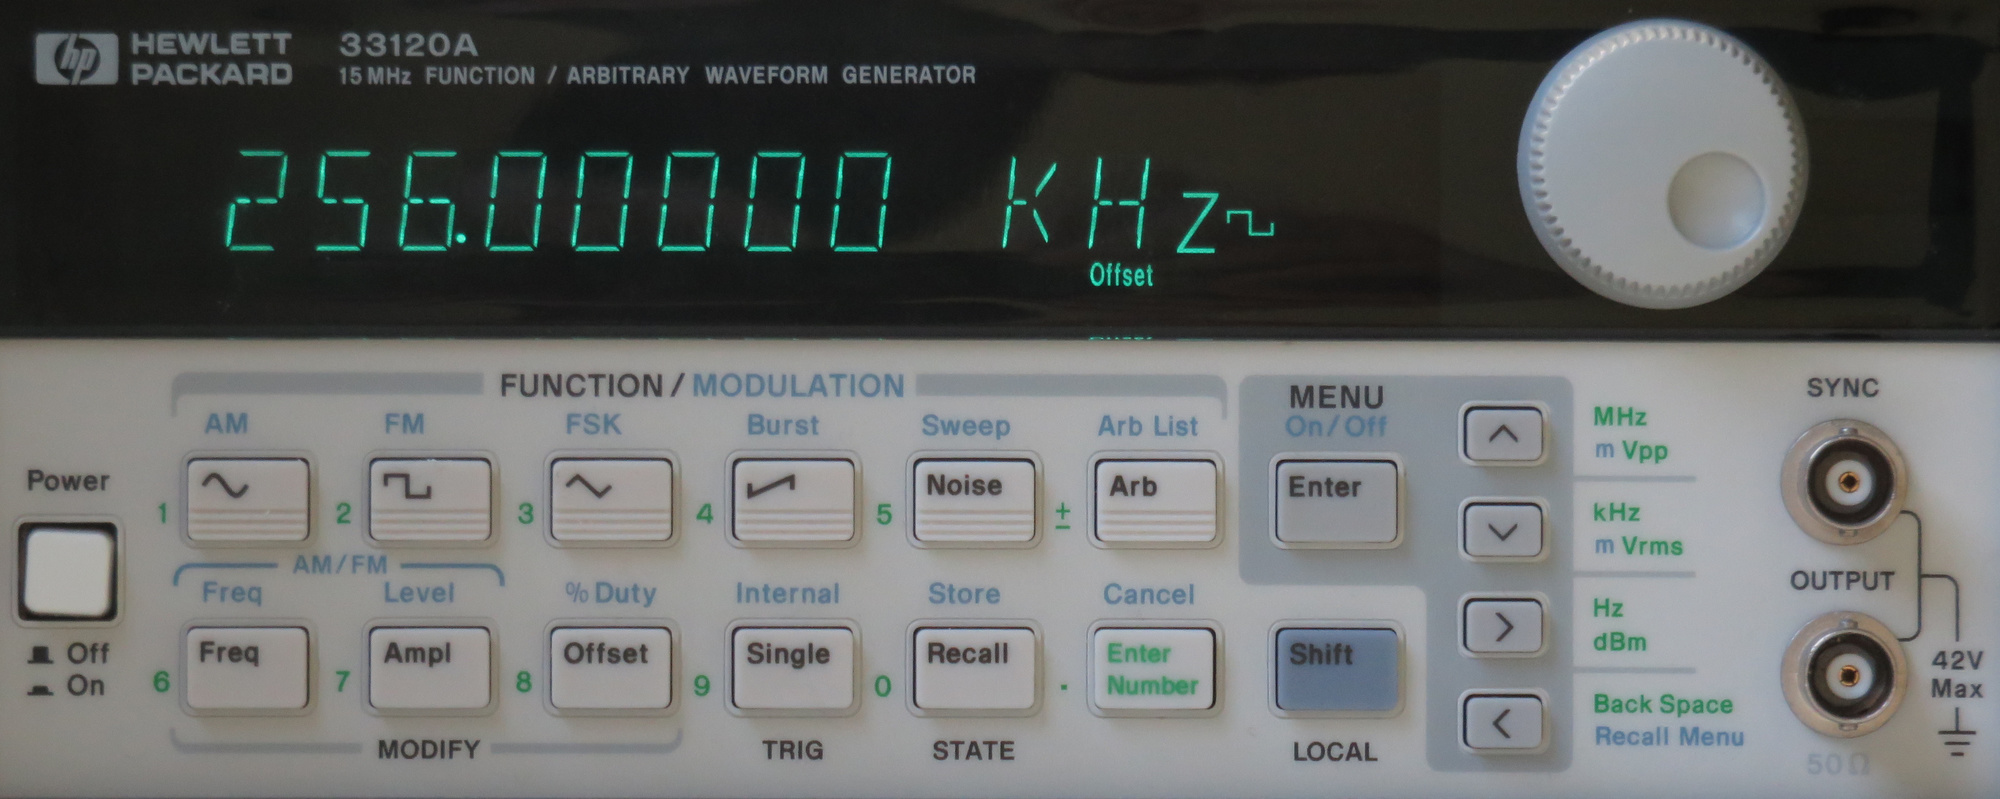
\includegraphics[width=0.67\textwidth]{images/funcGen/funcGen-12.jpg}
%    \caption{Initial screen after power-on}
%    \label{fig:HPwave:poweron}
%\end{figure}
